\chapter{RESULTADOS}

Os resultados obtidos com o desenvolvimento do OmniBot demonstram o êxito da proposta em integrar conceitos de robótica móvel, Internet das Coisas e controle distribuído.

Diante disso, este capítulo descreve como o robô a estrutura física do robô, como está funcionando atualmente, como testar os possíveis comandos e visualizar os dados que o robô disponibiliza. Também será apresentado os testes de controle de outras plataformas robóticas móveis terrestres físicas e simuladas com a solução IoT proposta com a BitDogLab e o ROS 2.

\section{ESTRUTURA FÍSICA E MONTAGEM}

A concepção do projeto iniciou-se pela modelagem tridimensional da estrutura do robô, desenvolvida no software Autodesk Fusion 360, onde foram definidos os parâmetros geométricos, pontos de fixação e o arranjo interno dos componentes, conforme apresentado na Figura \ref{fig:modelagem_omnibot}. Essa etapa foi essencial para prever o posicionamento dos motores, placas e sensores, além de otimizar a distribuição de massa e o espaço interno para manutenção.


\begin{figure}[!ht]
  \caption{\label{fig:modelagem_omnibot}Modelagem 3D do OmniBot no Autodesk Fusion 360 a) Vista interna b) Vista externa.}
  \centering
  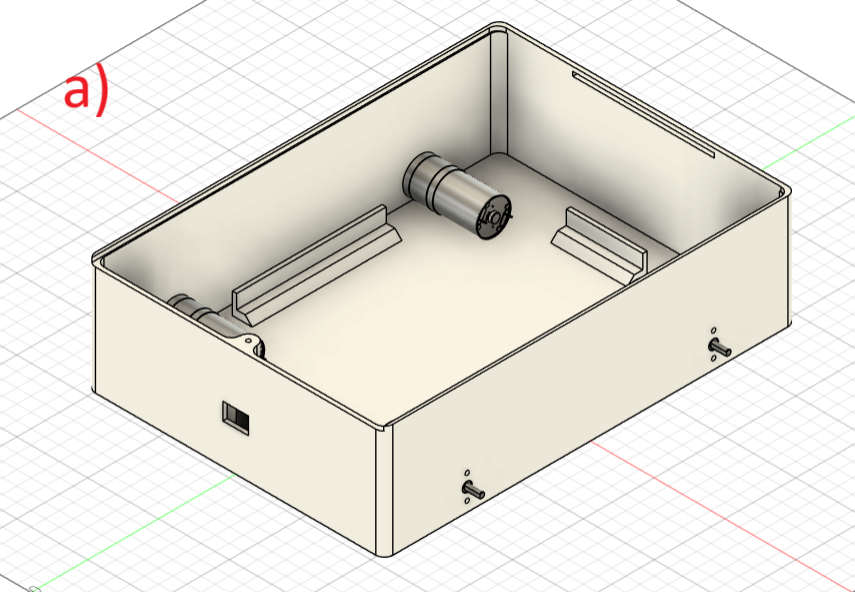
\includegraphics[scale=0.35]{figuras/modelagem_omnibot_interno.png}
  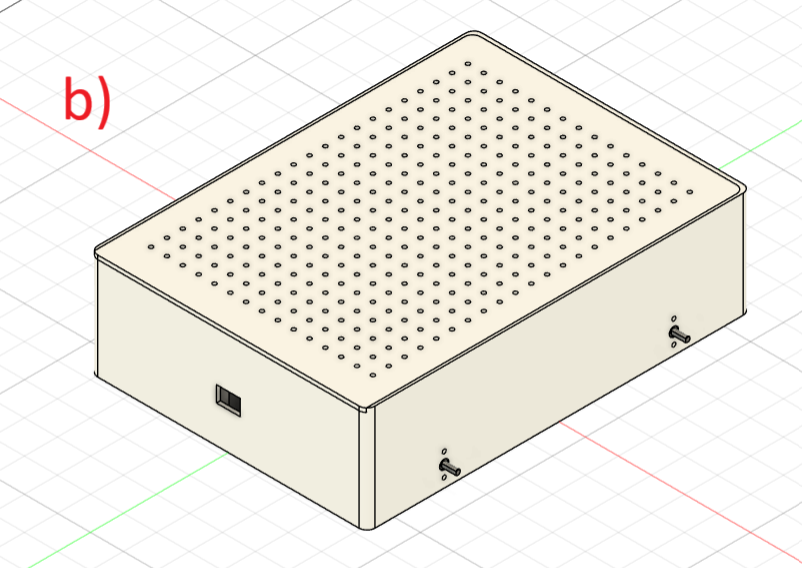
\includegraphics[scale=0.35]{figuras/modelagem_omnibot_externo.png}
  \legend{\Fonte{Elaborado pelo autor.}}
\end{figure}


Durante os testes práticos realizados no LABIRAS, a plataforma mostrou-se plenamente funcional, com os deslocamentos esperados em todas as direções possíveis. A matriz cinemática das rodas mecanum foi devidamente implementada, permitindo que o robô se movesse lateralmente, diagonalmente e rotacionasse sobre o próprio eixo sem perda de estabilidade. O controle de velocidade foi ajustado por meio de modulação PWM, garantindo suavidade nas transições.

A Figura \ref{fig:montagem_completa_omnibot} apresenta o OmniBot completamente montado, após a impressão das peças estruturais e a instalação dos sistemas eletrônicos e mecânicos.


\begin{figure}[!ht]
  \caption{\label{fig:montagem_completa_omnibot}Montagem física do robô OmniBot.}
  \centering
  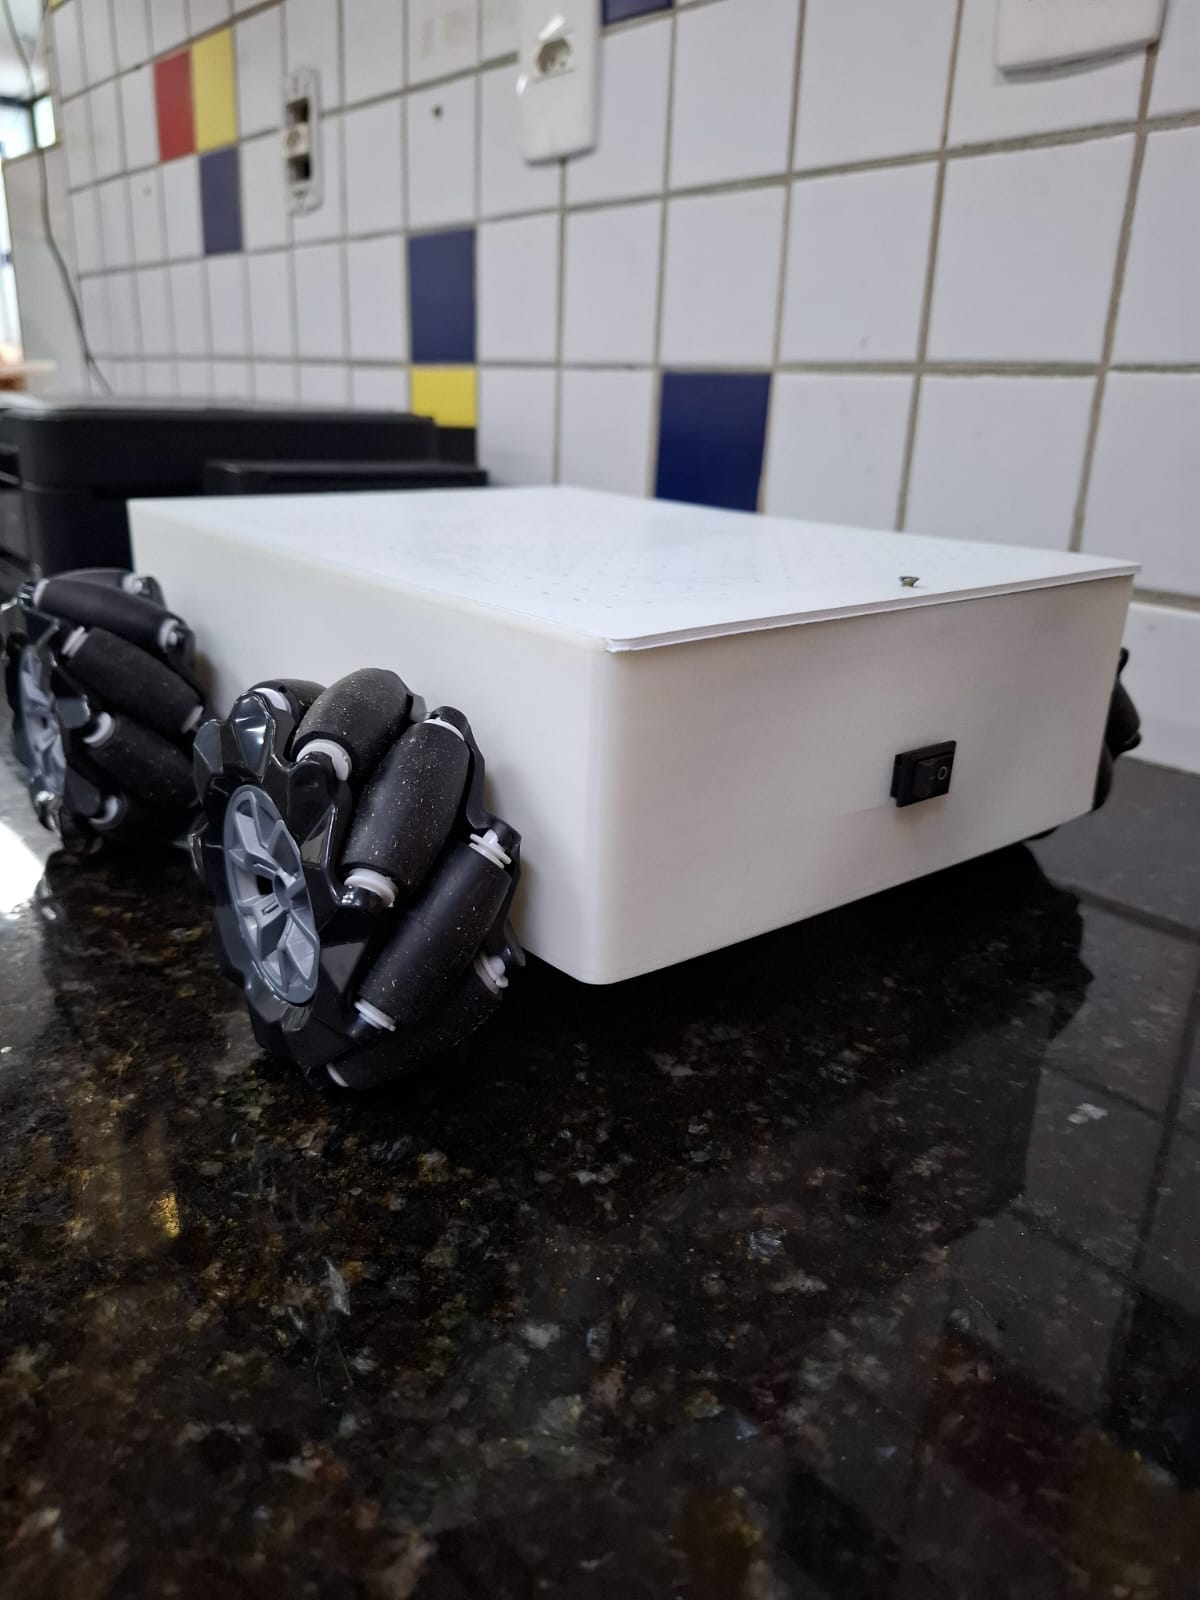
\includegraphics[scale=0.15]{figuras/montagem_completa_omnibot.jpg}
  \legend{\Fonte{Elaborado pelo autor.}}
\end{figure}


A comunicação entre o ESP32 e o ROS 2 Agent mostrou-se estável, onde o nó micro-ROS foi capaz de publicar informações de telemetria das rodas do robô (omnibot\_interfaces/Wheels) e receber comandos (geometry\_msgs/Twist) de forma contínua, validando a bidirecionalidade da arquitetura.

A placa de circuito impresso (PCB) desenvolvida para o projeto foi desenhada com o objetivo de organizar a ligação dos motores, \textit{encoders}, pontes H, microcontrolador e módulos de alimentação. A Figura \ref{fig:layout_pcb} apresenta o layout final da PCB, enquanto a Figura \ref{fig:diagrama_eletronico} exibe o diagrama esquemático do sistema eletrônico completo, mostrando a interligação entre o microcontrolador, drivers de motor e sensores.


\begin{figure}[!ht]
  \caption{\label{fig:layout_pcb}Layout da placa PCB de controle do OmniBot a) Vista superior b) Vista inferior.}
  \centering
  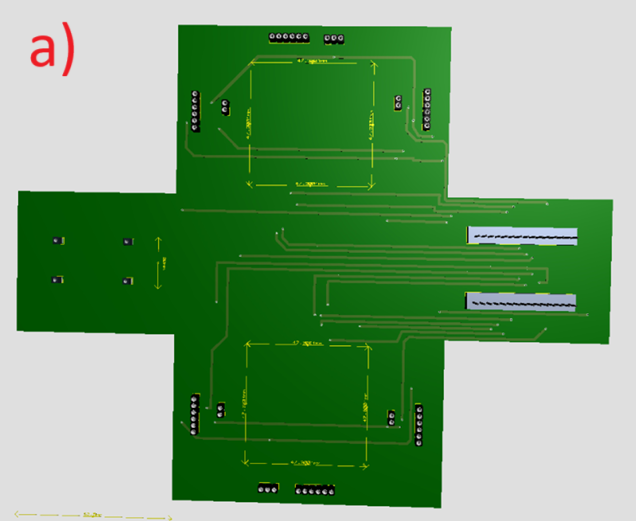
\includegraphics[scale=0.4]{figuras/PCB_Superior.png}
  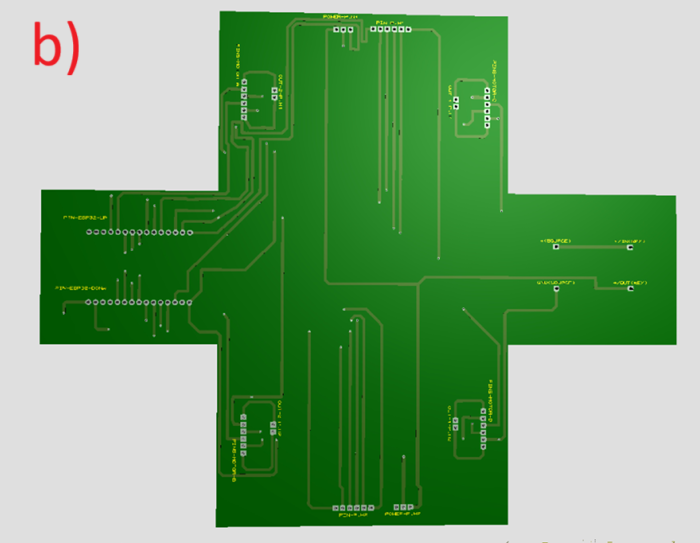
\includegraphics[scale=0.4]{figuras/PCB_Inferior.png}
  \legend{\Fonte{Elaborado pelo autor.}}
\end{figure}


\begin{figure}[!ht]
  \caption{\label{fig:diagrama_eletronico}Diagrama de esquemático conexões eletrônicas do OmniBot.}
  \centering
  \includegraphics[scale=0.5]{figuras/EsquematicoOmnibot.pdf}
  \legend{\Fonte{Elaborado pelo autor.}}
\end{figure}


Isto posto, a Figura \ref{fig:montagem_interna_omnibot} mostra a montagem interna do robô, evidenciando a fixação do microcontrolador ESP32 DevKit V1, da ponte H L298N, bem como das conexões de alimentação e sinal. A disposição foi planejada para facilitar a montagem e manutenção de componentes.


\begin{figure}[!ht]
  \caption{\label{fig:montagem_interna_omnibot}Montagem interna do OmniBot, mostrando o arranjo dos componentes.}
  \centering
  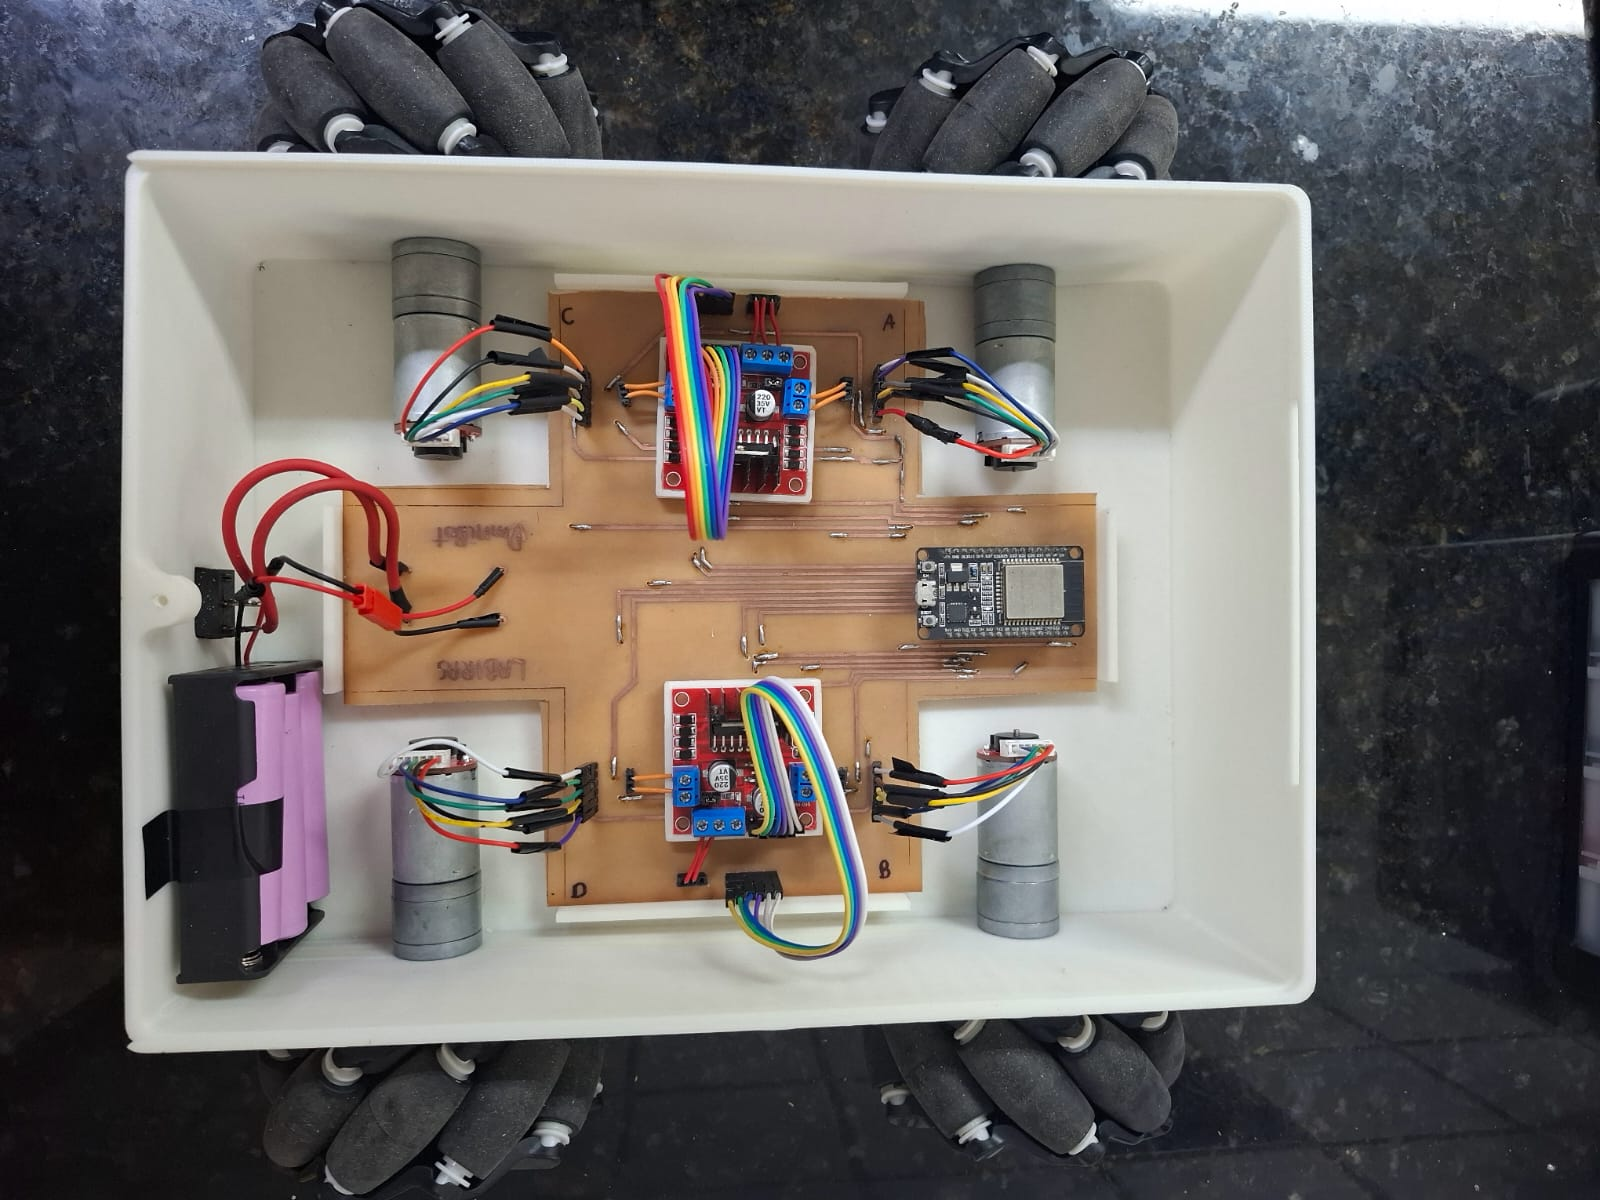
\includegraphics[scale=0.15]{figuras/montagem_interna_omnibot.jpg}
  \legend{\Fonte{Elaborado pelo autor.}}
\end{figure}


Para mais, a fim de acomodar a BitDogLab e permitir seu uso como controle portátil, foi projetado um case dedicado, também modelado no Fusion 360, que garante proteção física, ergonomia e praticidade no manuseio. A Figura \ref{fig:modelagem_case_bitdoglab} apresenta o modelo virtual do case, e a Figura \ref{fig:impressao_case_bitdoglab}, sua versão física impressa em 3D e acoplada a placa BitDogLab.


\begin{figure}[!ht]
  \caption{\label{fig:modelagem_case_bitdoglab}Modelagem do case desenvolvido para a BitDogLab.}
  \centering
  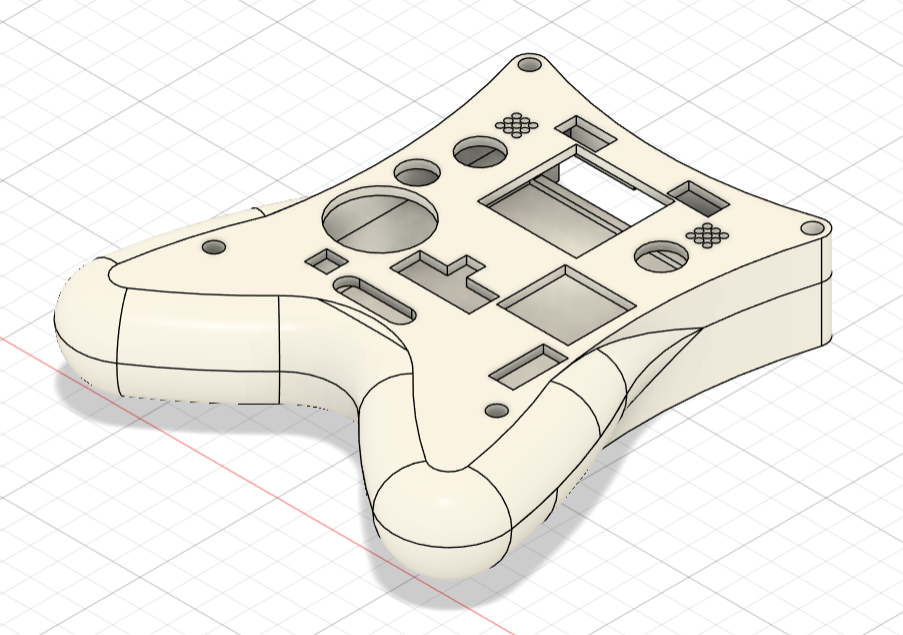
\includegraphics[scale=0.4]{figuras/modelagem_case_bitdoglab.png}
  \legend{\Fonte{Elaborado pelo autor.}}
\end{figure}


\begin{figure}[!ht]
  \caption{\label{fig:impressao_case_bitdoglab}Case da BitDogLab impresso em 3D a) Vista frontal b) Vista posterior.}
  \centering
  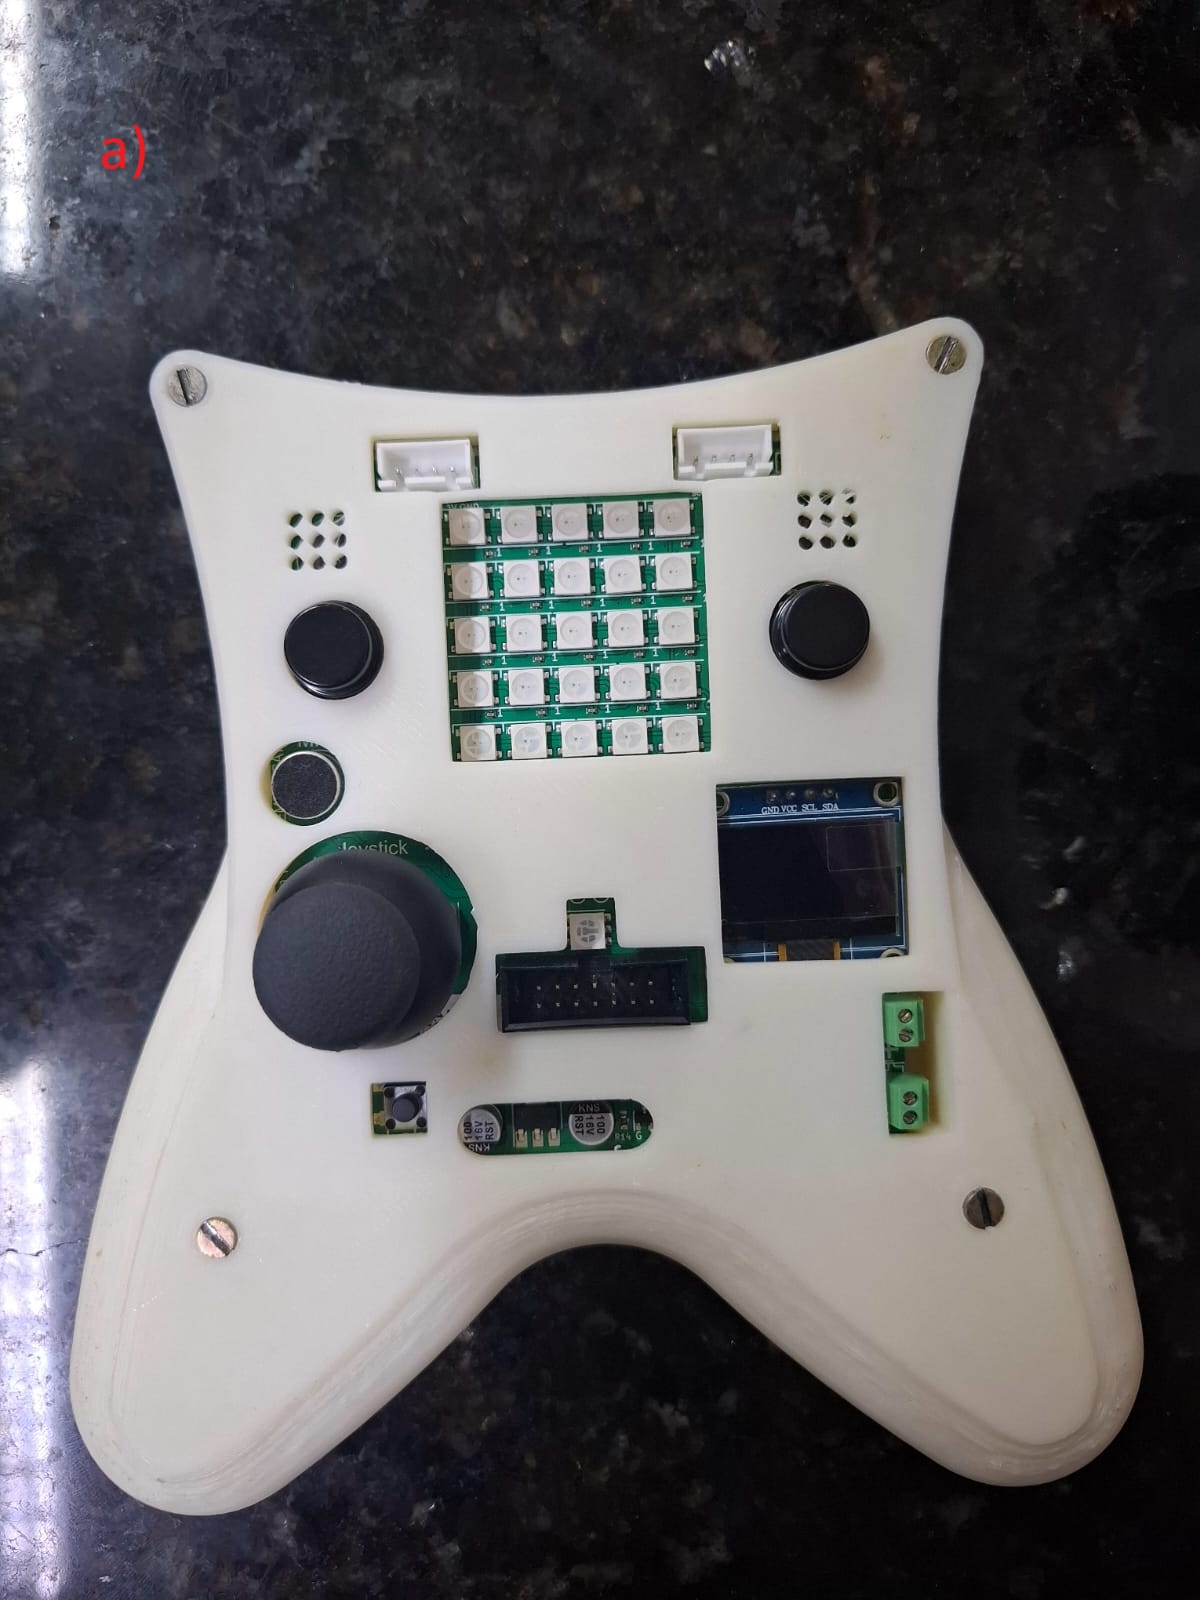
\includegraphics[scale=0.15]{figuras/impressao_case_bitdoglab_frontal.jpg}
  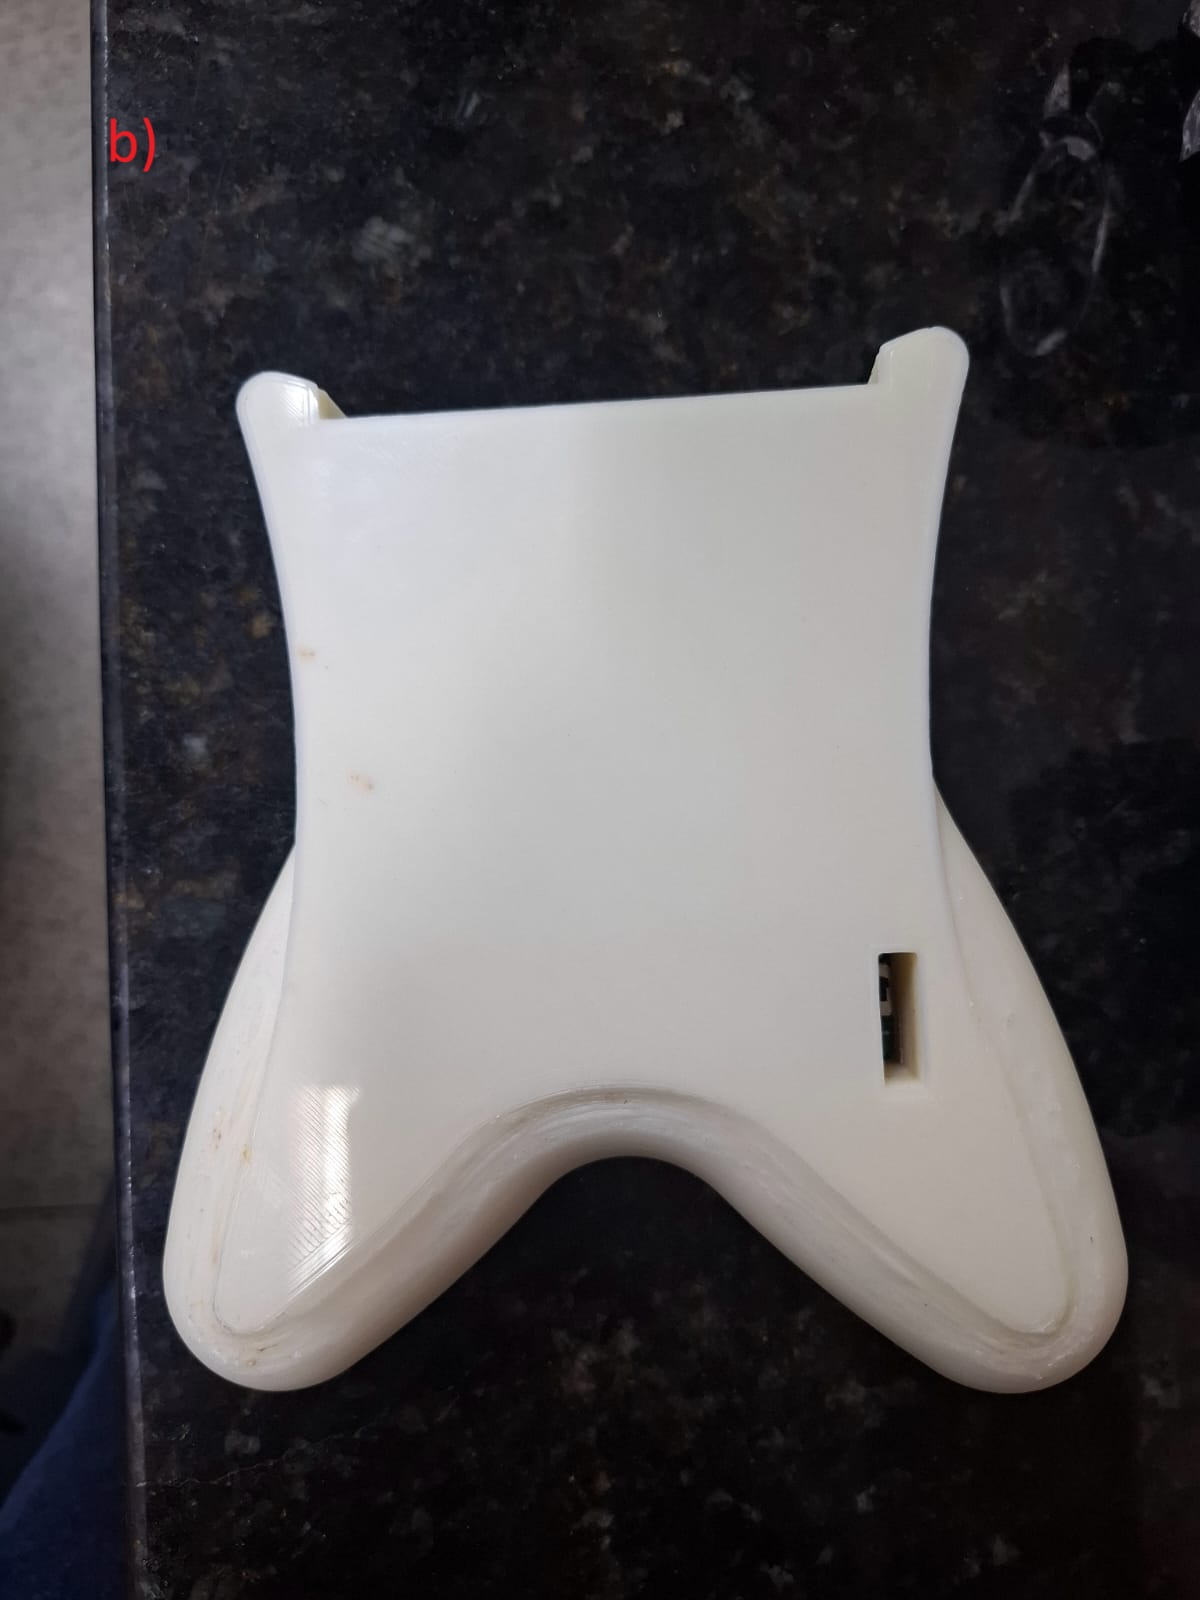
\includegraphics[scale=0.15]{figuras/impressao_case_bitdoglab_posterior.jpg}
  \legend{\Fonte{Elaborado pelo autor.}}
\end{figure}


Em termos de construção, o chassi impresso em 3D, bem como o case da placa BitDogLab, apresentaram resistência adequada às solicitações mecânicas e facilidade de manutenção. A modularidade do projeto possibilitou a substituição de componentes sem necessidade de reconstrução integral da estrutura, reforçando o caráter educacional da plataforma.




\section{OPERAÇÃO DO ROBÔ}

Para a inicialização do robô, é necessário que o \textit{micro-ROS Agent} esteja executando na máquina, a qual o endereço IP foi configurado no algoritmo do robô, e ambos estejam configurados na mesma rede, conforme exposto na Figura \ref{fig:configuracao_parametros_omnibot}. O \textit{micro-ROS Agent} pode ser instalado criando um \textit{ROS workspace} e clonando o \textit{package} \textit{micro\_ros\_setup} e compilando manualmente, ou utilizando uma imagem \textit{Docker} como mostra \citeonline{dockeresp32}, onde adotou-se a primeira opção.


\begin{figure}[!ht]
  \caption{\label{fig:configuracao_parametros_omnibot}Configuração dos parâmetros do robô.}
  \centering
  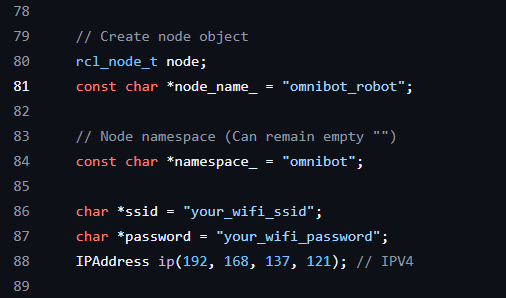
\includegraphics[scale=0.8]{figuras/configuracao_parametros_omnibot.png}
  \legend{\Fonte{Elaborado pelo autor.}}
\end{figure}


Após a conexão, o \textit{Agent} cria o \textit{node} e os \textit{topics}, podendo ser visualizados usando a ferramenta \textit{rqt\_graph} do ROS (Figura \ref{fig:rqt}). São dois \textit{topics} e um \textit{node}, todos possuindo o prefixo do \textit{namespace} que foi definido nos parâmetros do robô. Nesse caso o \textit{namespace} é \textbf{/omnibot}.


\begin{figure}[!ht]
    \Caption{\label{fig:rqt}rqt mostrando o \textit{node} e \textit{topics} gerados pelo micro-ROS.}
    \centering
    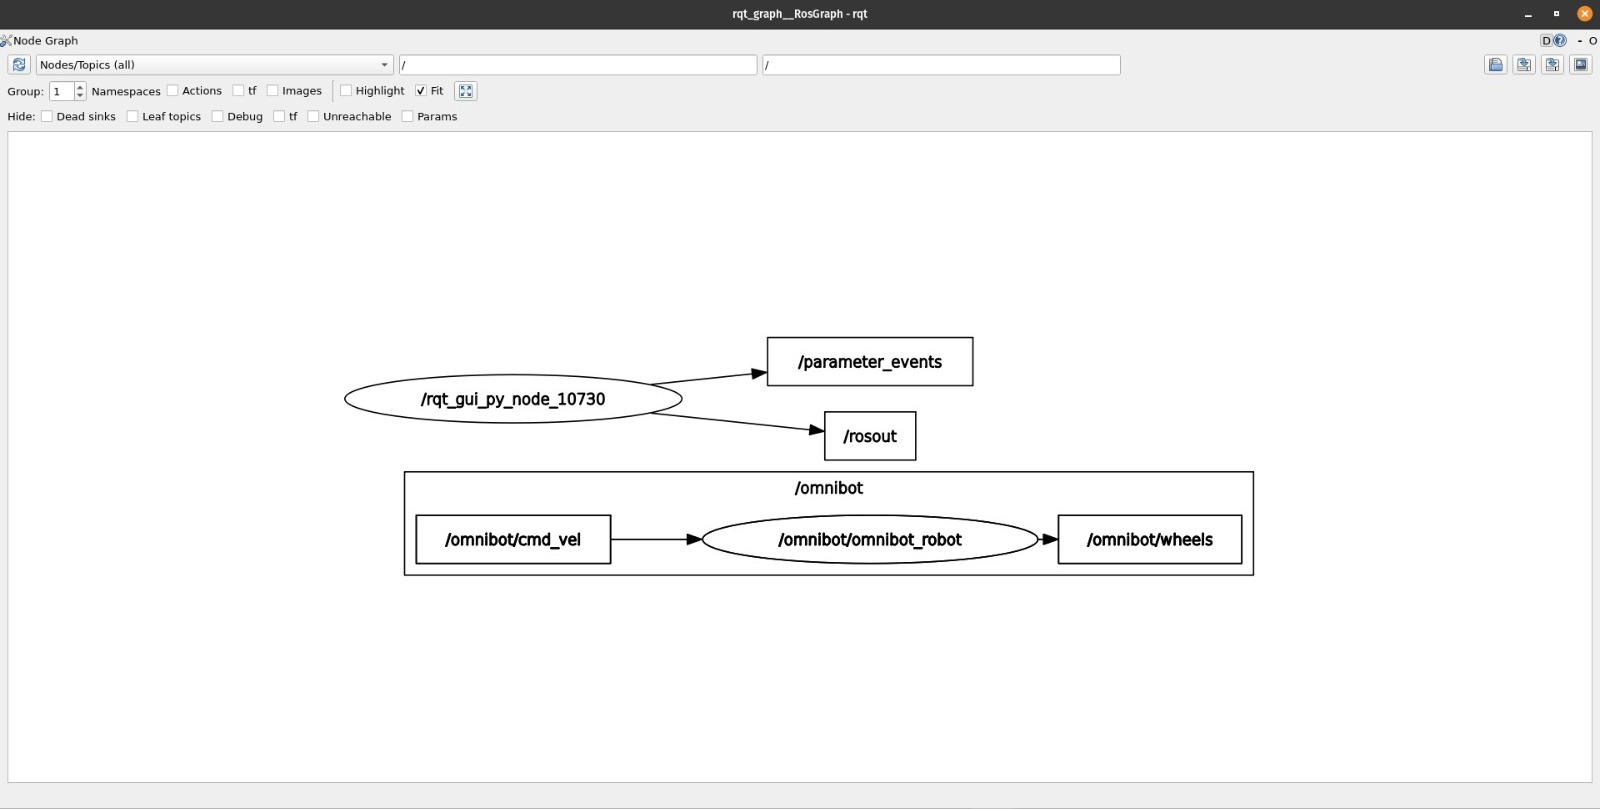
\includegraphics[scale=0.25]{figuras/rqt_sem_http_node.jpg}
    \legend{\Fonte{Elaborado pelo autor.}}
\end{figure}


Para movimentação o ESP32 espera mensagens do tipo \textbf{geometry\_msgs/msg/Twist} no \textit{topic} \textbf{/omnibot/cmd\_vel}. A mensagem é definida por dois vetores de velocidade, um linear com x, y e z, e um angular também com x, y e z. O robô só consegue se mover no plano, andando nas direções x e y, e rotacionando em z. Sendo assim, só as componentes lineares x e y, e angular z serão necessárias. O ESP32 espera esses valores e comanda os motores de acordo.

Essa estrutura demostra que o OmniBot é capaz de ser operado tanto em modo manual, quanto remoto, a partir de uma interface ROS, o que viabiliza futuras aplicações em ambientes distribuídos.

Ainda assim, para publicar em \textbf{/omnibot/cmd\_vel} foi utilizado o \textit{node} desenvolvido em C++ que funciona como \textit{middleware} ROS 2 de comunicação entre o robô e a placa BitDogLab. Esse \textit{node} cuida de receber os comandos via requisições HTTP da placa de controle e transformar em mensagens pdo tipo \textbf{geometry\_msgs/msg/Twist} para serem enviadas ao Omnibot através do tópico especificado, bem como retornar a BitDogLab os dados dos \textit{encoders} do robô provenientes do tópico \textbf{/omnibot/wheels}. Após a inicialização desse \textit{node}, a estrutura de nós e tópicos ROS ficam conforme exposto pela ferramenta rqt da Figura \ref{fig:rqt}.


\begin{figure}[!ht]
    \Caption{\label{fig:rqt}rqt mostrando toda a arquitetura de conexão dos \textit{nodes} e \textit{topics}.}
    \centering
    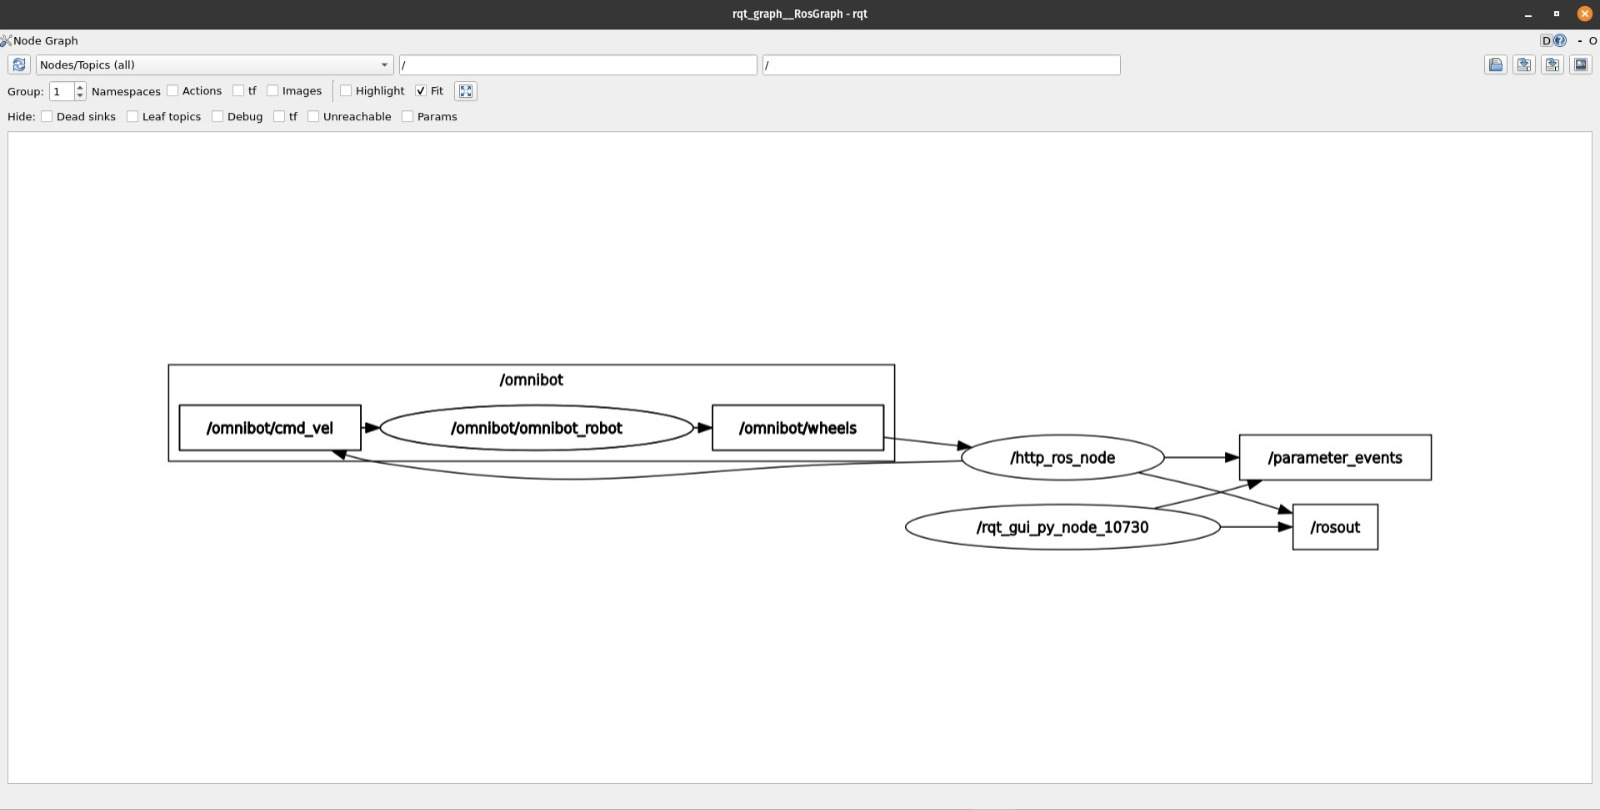
\includegraphics[scale=0.25]{figuras/rqt_com_http_node.jpg}
    \legend{\Fonte{Elaborado pelo autor.}}
\end{figure}


O \textit{node} desenvolvido gerencia de forma dinâmica a descoberta e exclusão de robôs móveis controláveis. Isso é possível através de uma busca por todos os tópicos com terminação \textbf{cmd\_vel} e \textbf{wheels}, e por uma análise se há \textit{subscribers} nesses tópicos \textbf{cmd\_vel} e se há \textit{publishers} nos tópicos com \textbf{wheels}. Através dessa busca, é possível identificar novos robôs conectados ao ROS e robôs que foram desconectados, podendo assim gerenciar dinamicamente os dispositivos.

Dessa forma, a quantidade e o dispositivo robótico que será controlado podem ser visualizados através da IHM exibida pela tela OLED da BitDogLab, bem como as informações das leituras dos \textit{encoders} das rodas do robô e dos dados da mensagem cmd\_vel (linear x e y, e angular z), conforme elucidado na Figura \ref{fig:display_oled_bitdoglab}.


\begin{figure}[!ht]
    \Caption{\label{fig:display_oled_bitdoglab}Informações do display OLED da BitDogLab do funcionamento em a) Modo diferencial b) Modo holonômico.}
    \centering
    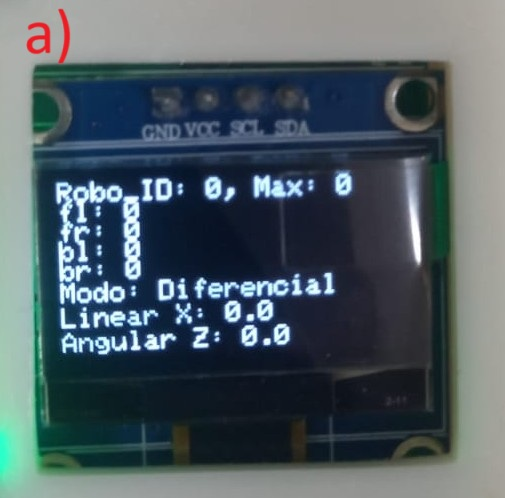
\includegraphics[scale=0.4]{figuras/display_bitdoglab_diferencial.jpg}
    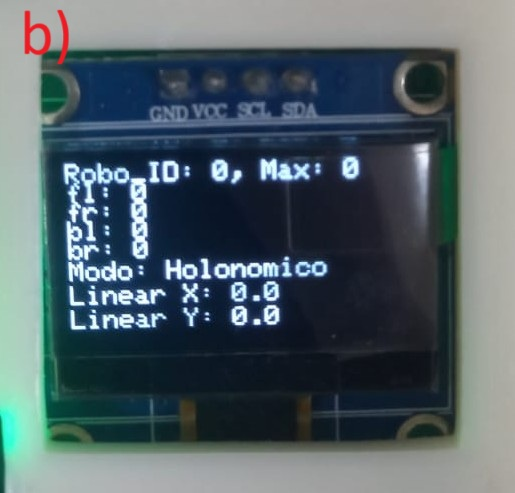
\includegraphics[scale=0.4]{figuras/display_bitdoglab_holonomico.jpg}
    \legend{\Fonte{Elaborado pelo autor.}}
\end{figure}


Diante disso, assim como \citeonline{vilanova2022aeronave}, verifica-se a possibilidade de uso da plataforma robótica elaborada como recurso didático para aplicação dos conteúdos de controle, automação e sistemas embarcados, integrando sensores, atuadores e comunicação em rede em um ambiente real de aprendizagem.

No mais, análogo a \citeonline{ramalho2020omnino}, obteve-se os mesmos princípios de modularidade, acessibilidade e interoperabilidade, mas com foco em aplicações educacionais e integração IoT para controle remoto e monitoramento via rede sem fio. Outro ponto, diferente de \citeonline{ramalho2020omnino}, montou-se uma plataforma robótica omnidirecional com arquitetura de 4 rodas \textit{mecanum}, mas que também apresenta compatibilidade com o ROS 2.


\section{OPERAÇÃO DE OUTRAS PLATAFORMAS ROBÓTICAS}

Com a arquitetura desenvolvida do projeto, conforme destacado na Figura \ref{fig:diagrama_conexoes_dispositivos}, foi possível estabelecer conexão com outras plataformas robóticas móveis, físicas e simuladas.

Através do \textit{node} ROS 2 desenvolvido, obteve-se validação de controle da plataforma robótica móvel terrestre
diferencial do laboratório LABIRAS, desenvolvida com base no Roomba® 614 iRobot. Durante os testes, foi possível controlar a movimentação da mesma através da solução Iot elaborada, bem como coletar os dados dos \textit{encoders} de suas rodas e disponibilizar na IHM elaborada.

Outrossim, o teste estendeu-se em validar, ao mesmo tempo, o controle de plataformas robóticas móveis terrestres simuladas. Para tal, utilizou-se o Turtlesim, um simulador de aprendizado ROS 2, também obtendo resposta positiva. Nas Figuras \ref{fig:rqt_multiplos} e \ref{fig:display_oled_bitdoglab_multiplos} são expostas a estrutura de nós e tópicos ROS através da ferramenta rqt e a IHM exibida pela tela OLED da BitDogLab, respectivamente, durante a operação desses 3 dispositivos de forma simultânea.


\begin{figure}[!ht]
    \Caption{\label{fig:rqt_multiplos}rqt mostrando toda a arquitetura de conexão dos \textit{nodes} e \textit{topics} para operação simultânea de 3 dispositivos robóticos.}
    \centering
    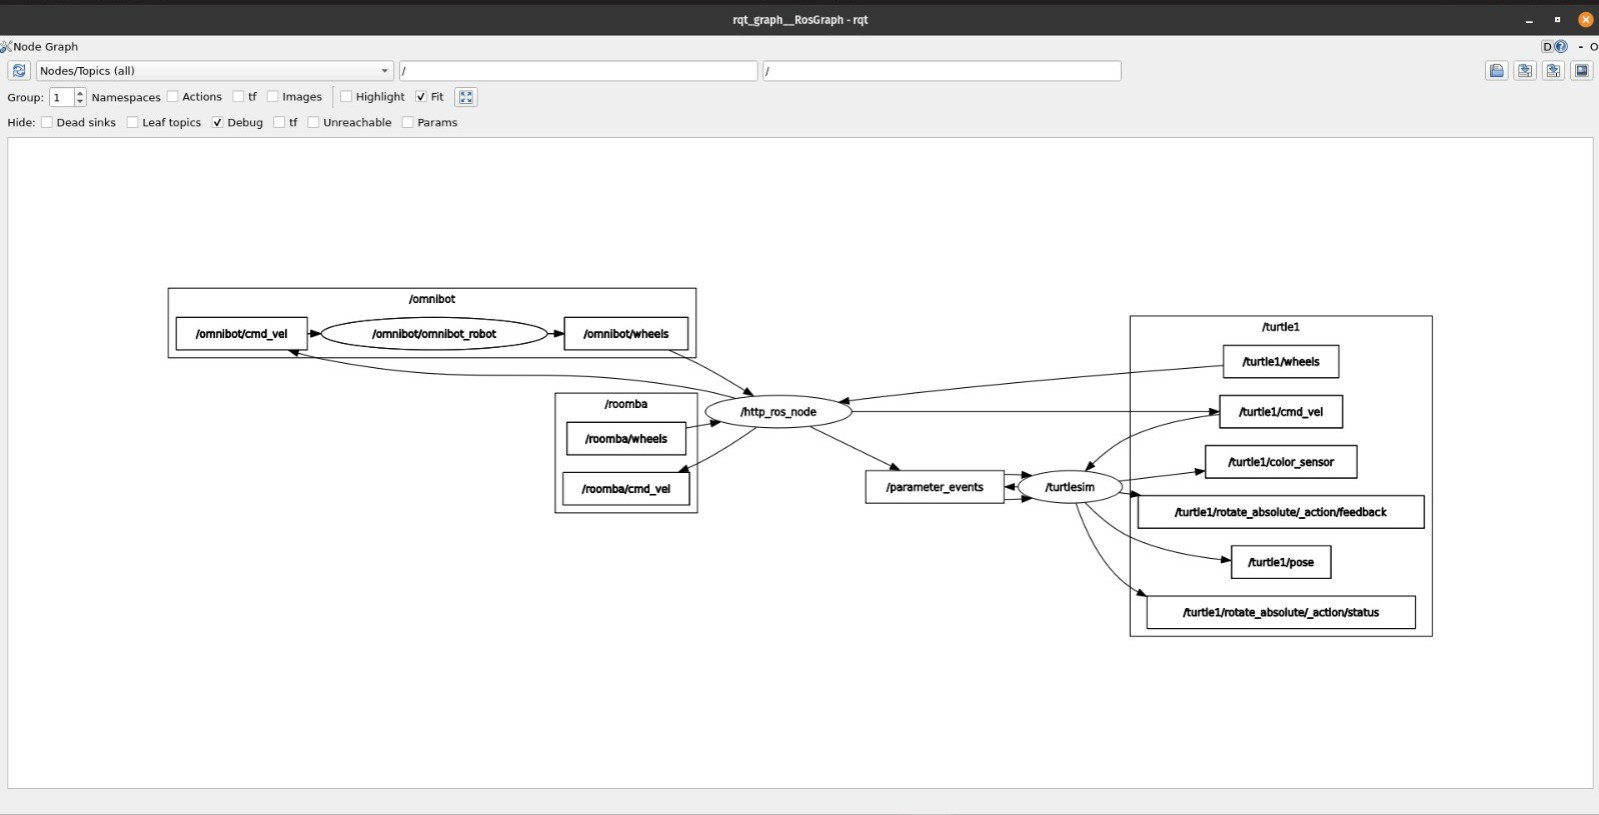
\includegraphics[scale=0.23]{figuras/rqt_multiplos_robos.jpg}
    \legend{\Fonte{Elaborado pelo autor.}}
\end{figure}


\begin{figure}[!ht]
    \Caption{\label{fig:display_oled_bitdoglab_multiplos}Informações do display OLED da BitDogLab do funcionamento durante a operação simultânea de 3 dispositivos robóticos em a) Modo diferencial b) Modo holonômico.}
    \centering
    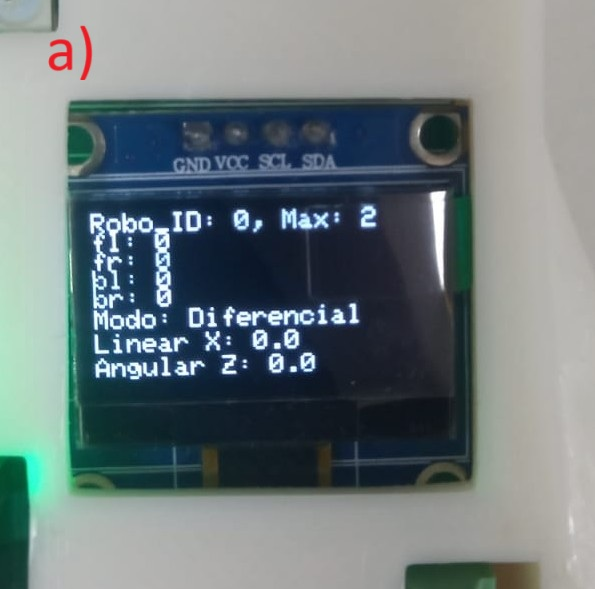
\includegraphics[scale=0.4]{figuras/display_bitdoglab_diferencial_multiplos.jpg}
    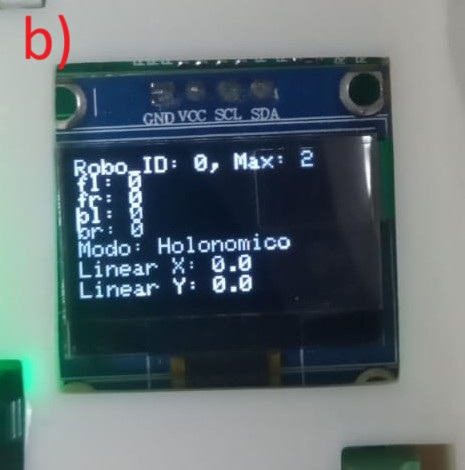
\includegraphics[scale=0.5]{figuras/display_bitdoglab_holonomico_multiplos.jpg}
    \legend{\Fonte{Elaborado pelo autor.}}
\end{figure}

Destarte, assim, o controle remoto via BitDogLab apresentou desempenho satisfatório em termos de responsividade e confiabilidade da transmissão. Além disso, a tela OLED exibiu corretamente os parâmetros de conexão e as informações acerca dos \textit{encoders} do robô em tempo real, oferecendo ao operador um feedback constante durante a operação.

Esses resultados indicam que o sistema é uma ferramenta eficiente para o ensino de conceitos como cinemática, controle e integração de sistemas embarcados com IoT, atendendo plenamente aos objetivos propostos.
